\section{Gaussian Merging}
As discussed in the previous chapter, one way to accelerate 3DGS rendering is by reducing the number of primitives in the scene, which can be done using simplified representations, similar to levels-of-detail on triangle meshes. Some implementations presented in the literature review propose very simple methods for Gaussian merging, such as averaging all properties. This technique is not accurate for all properties, but in those cases, it is a good starting point, as the simplified representations are also trained during the scene optimization process. However, for this implementation, I need to find an approach that produces quality results without further fine-tuning, because the simplifications are used directly as they are generated at runtime. In this chapter, I will present the approach used in this implementation for merging two Gaussian into one primitive in order to obtain scene representations with fewer Gaussians.

\subsection{Spherical Harmonics}
The main use of the merged Gaussians is to replace primitives far away from the camera with a simplified representation in order to increase performance by decreasing detail in areas where the loss in quality is not that noticeable. Thus, the intended use of the simplification is distant areas from the camera. In this situation, the original Gaussians will only take up a reduced area on the screen, which would be equivalent to rendering them at a lower resolution if they were closer to the camera. Using the insight from studies on antialiasing for Gaussian splatting, a good option for band-limiting the rendered primitives is to apply a box blur filter that acts as a low-pass filter. Applying a 2D box blur filter to a patch of pixels on the screen is done by convolution of the initial image with a $3 \times 3$ kernel with the following formulation when applied in image space \cite{box_filter}: 
\[H = \frac{1}{9} \begin{bmatrix}
1 & 1 & 1\\
1 & 1 & 1\\
1 & 1 & 1
\end{bmatrix}\]

As expected, the blur used to subsample the projected primitives to improve aliasing takes the average of neighboring pixels. That indicates that in order to get a similar representation from a single primitive, a good choice for the color is the mean of the initial primitives. However, taking a simple average of the color would ignore the different contributions different Gaussians have to the final image on the screen. Some implementations propose determining the visual importance of a Gaussian as the amount of overlapped pixels over all training images. While this is a relevant metric, the method I am proposing is intended for generic use on 3DGS scenes, not necessarily aiming for the highest metrics on a set of predetermined camera positions. For this reason, I chose to consider the relative contribution of a Gaussian as a function of its learned opacity and volume. Thus, I chose the following formulation to define the weight of a Gaussian $i$: $w_i = \alpha_i \cdot V_i$, where $V_i = s_x\cdot s_y \cdot s_z$. Because the actual color is computed in every frame depending on the camera position, I will blend the Gaussians using a weighted mean on the arrays of SH coefficients. The coefficients are separated by color, so the weighted mean can be applied to each channel individually and will provide the desired result when recomposing the color from the new SH coefficients and viewing direction. 

\subsection{Opacity}
In order to compute the opacity of the merged Gaussian, I am using an approach similar to the one in \cite{kerbl_hierarchy}. One thing to note is that the opacity property of Gaussians defines the maximum opacity at the center of the splat and is the value from which the splat's opacity falls following a Gaussian curve towards the edges of the splat. However, when two Gaussians projected to the screen overlap, the perceived opacity across them does not follow a Gaussian distribution, as the two opacities are composed over the overlapping region, so the falloff is slower than a Gaussian. 

\begin{wrapfigure}{r}{5.5cm}
    \centering
    \includesvg[width=\linewidth]{figures/blending.svg}
    \caption{Scanlines across the initial Gaussians and the merged one.}
    \label{fig:blendfig}
\end{wrapfigure}

It is important to model this behavior, otherwise the merged primitive will have lower perceived opacity, and applying the merging procedure hierarchically would result in significant opacity loss across the scene. Consider two partially overlapping Gaussians projected on the screen as in figure \ref{fig:blendfig}. A scanline plotting the opacities across the space occupied by the two splats will produce the profiles shown below, where figure \ref{fig:opacity_sum} shows the sum of opacities generated by the distributions, and figure \ref{fig:perceived_opacity} shows the total opacity saturated at 1, as that is the maximum opacity accepted by the rasterization routine. Note the plateau around the center of the two splats generated by the sum of the two decaying opacities, which cannot be directly modeled by a Gaussian distribution. 

However, the shape of the function above the $\alpha = 1$ line is not important, as the opacity will be saturated at 1. This means that this behavior can be modeled by a single Gaussian distribution with a peak higher than 1, as shown in figure \ref{fig:merged_model}. This is an oversimplification of the potential situations for Gaussian opacity merging, and the height of the distribution would depend on many variables such as the distance between primitives and their scales. However, it showcases the need for primitives after merging to have an opacity greater than 1 to simulate a slower fall-off.

\begin{figure}[H]
\makebox[\textwidth][c]{
    \centering
    \begin{minipage}{0.4\textwidth}
        \centering
        \includesvg[width=\linewidth]{figures/opacity_sum.svg}
        \caption{Scanline opacities.}
        \label{fig:opacity_sum}
    \end{minipage}\hfill
    \begin{minipage}{0.4\textwidth}
        \centering
        \includesvg[width=\linewidth]{figures/perceived_opacity.svg}
        \caption{Perceived opacity.}
        \label{fig:perceived_opacity}
    \end{minipage}\hfill
    \begin{minipage}{0.4\textwidth}
        \centering
        \includesvg[width=\linewidth]{figures/merged_model.svg}
        \caption{Merged opacity model.}
        \label{fig:merged_model}
    \end{minipage}
    }
\end{figure}

I chose to use a similar approach to the \textit{Hierarchical 3D Gaussian Representation} paper from INRIA, but changing the splat surface to Gaussian volume, as it would be a more reliable metric for any arbitrary view in the scene. Thus, the opacity of a merged Gaussian is the following:
\[
\alpha_m = \frac{\sum_i^N w_i}{V_m}
\]
where $V_m$ is the volume of the new Gaussian from its covariance matrix, as will be explained in the next subchapter, the weights $w_i$ are the same as for the color merging.

\subsection{Mean and Covariance}
The most difficult properties to merge for Gaussian primitives are the geometric ones, such as mean and covariance. Especially the covariance, it defines both the spread of the distribution and its directions, i.e. the orientation of the Gaussian in space. A lot of research has gone into reducing the dimensionality of Gaussian Mixture Models, both from a purely analytical perspective \cite{gaussmerge2} and for use in hierarchical photon mapping \cite{gaussmerge1}. Considering any arbitrary normalized weights $w_i'$ assigned to a set of N Gaussians, the mean and covariance of the merged Gaussian are the following:
\[
\overline{\mu} = \sum_{i \leq N} w_i' \mu_i
\]
\[
\overline{\Sigma} = \sum_{i \leq N} w_i'(\Sigma_i + (\mu_i - \overline{\mu}) (\mu_i - \overline{\mu})^T) 
\]

This method aims to minimize the Kullback–Leibler divergence, which measures how much two probability distributions differ. The formulas above are also used by \cite{kerbl_hierarchy} to generate their intermediary nodes, but note that the scene training algorithm then optimizes the generated nodes. During testing, I implemented this merging approach but found that a direct implementation of the formulas above results in Gaussians that have lower volume than expected, so applying the same approach on multiple levels resulted in significant gaps appearing in the scene. Note that at the time of writing, the implementation of \cite{kerbl_hierarchy} was not published, so there was no reference to any pre- or post-processing they are doing to achieve the results described. Also, their very good quality metrics are very likely to be due to the extended training process after the merged Gaussians are generated.

In order to test an alternative to the method above, I chose to implement a covariance merging approach based on the volumetric coverage of the combined Gaussians. The challenge when merging primitives is to get a similar shape to the initial distributions and fill in the same space occupied by them. To achieve this, I chose to follow an approach that analyzes the volumetric extent of the composed Gaussians and tries to reproduce the same volumetric coverage using only one distribution. 

Given a set of $N$ 3D Gaussian distributions, the first step is to determine their volumetric coverage, which is the space they occupy inside their 99\% confidence interval. I chose to use this interval as it is the same one that is used after the primitives are projected to determine their on-screen bounds. From the eigenvectors of the covariance matrix, we can determine the axes of the confidence ellipsoid, and by scaling these vectors by a factor of 3, we get the extent needed to cover the desired confidence interval. Given the scaled vectors $\bm{s_1}, \bm{s_2}, \bm{s_3}$ that represent the ellipsoid axes and the center point of the Gaussian $\bm{\mu}$, I can generate a coverage point cloud $P$ defined as 
\[P = \{\bm{\mu}, \bm{\mu} + \bm{s_1}, \bm{\mu} + \bm{s_2}, \bm{\mu} + \bm{s_3}, \bm{\mu} - \bm{s_1},\bm{ \mu} - \bm{s_2}, \bm{\mu} - \bm{s_3}\}\]
which contains the center point and the ellipsoid vertices. This procedure is applied to all the primitives that are going to be merged, then we concatenate the sets of points generated by them:
\[Q = \bigcup_{i=1}^N P_i\]
The final volumetric coverage point set will contain $7N$ points. To get the merged Gaussian mean, we will take the weighted average of these positions, the weights being the same as for the other properties before:
\[
\bm{\overline{\mu}} = \frac{1}{\sum_i^{7N} w_i} \sum_{\bm{p} \in Q} w_p\bm{p} 
\]

The weights for all 7 points generated by one Gaussian are the same. Then, to compute the equivalent Gaussian spread, we only need to compute the covariance of the point set. Let the matrix $D \in \mathbb{R}^{7N \times 3}$ be defined as:
\[
D_i = Q_i - \bm{\overline{\mu}}, 1 \leq i \leq 7N
\]
and the diagonal weight matrix $W = diag(\bm{w}) \in \mathbb{R}^{7N \times 7N}$. Then, the weighted covariance matrix \cite{weighted_mean} is defined as:
\[
\Sigma = \bm{DWD^T}
\]

With the two formulas above we have the necessary information to describe the new distribution. Figure 1 shows a simplified 2D representation of the coverage points and the computed resulting distribution for four Gaussians placed in different configurations in space.

\begin{figure}[H]
    \centering
    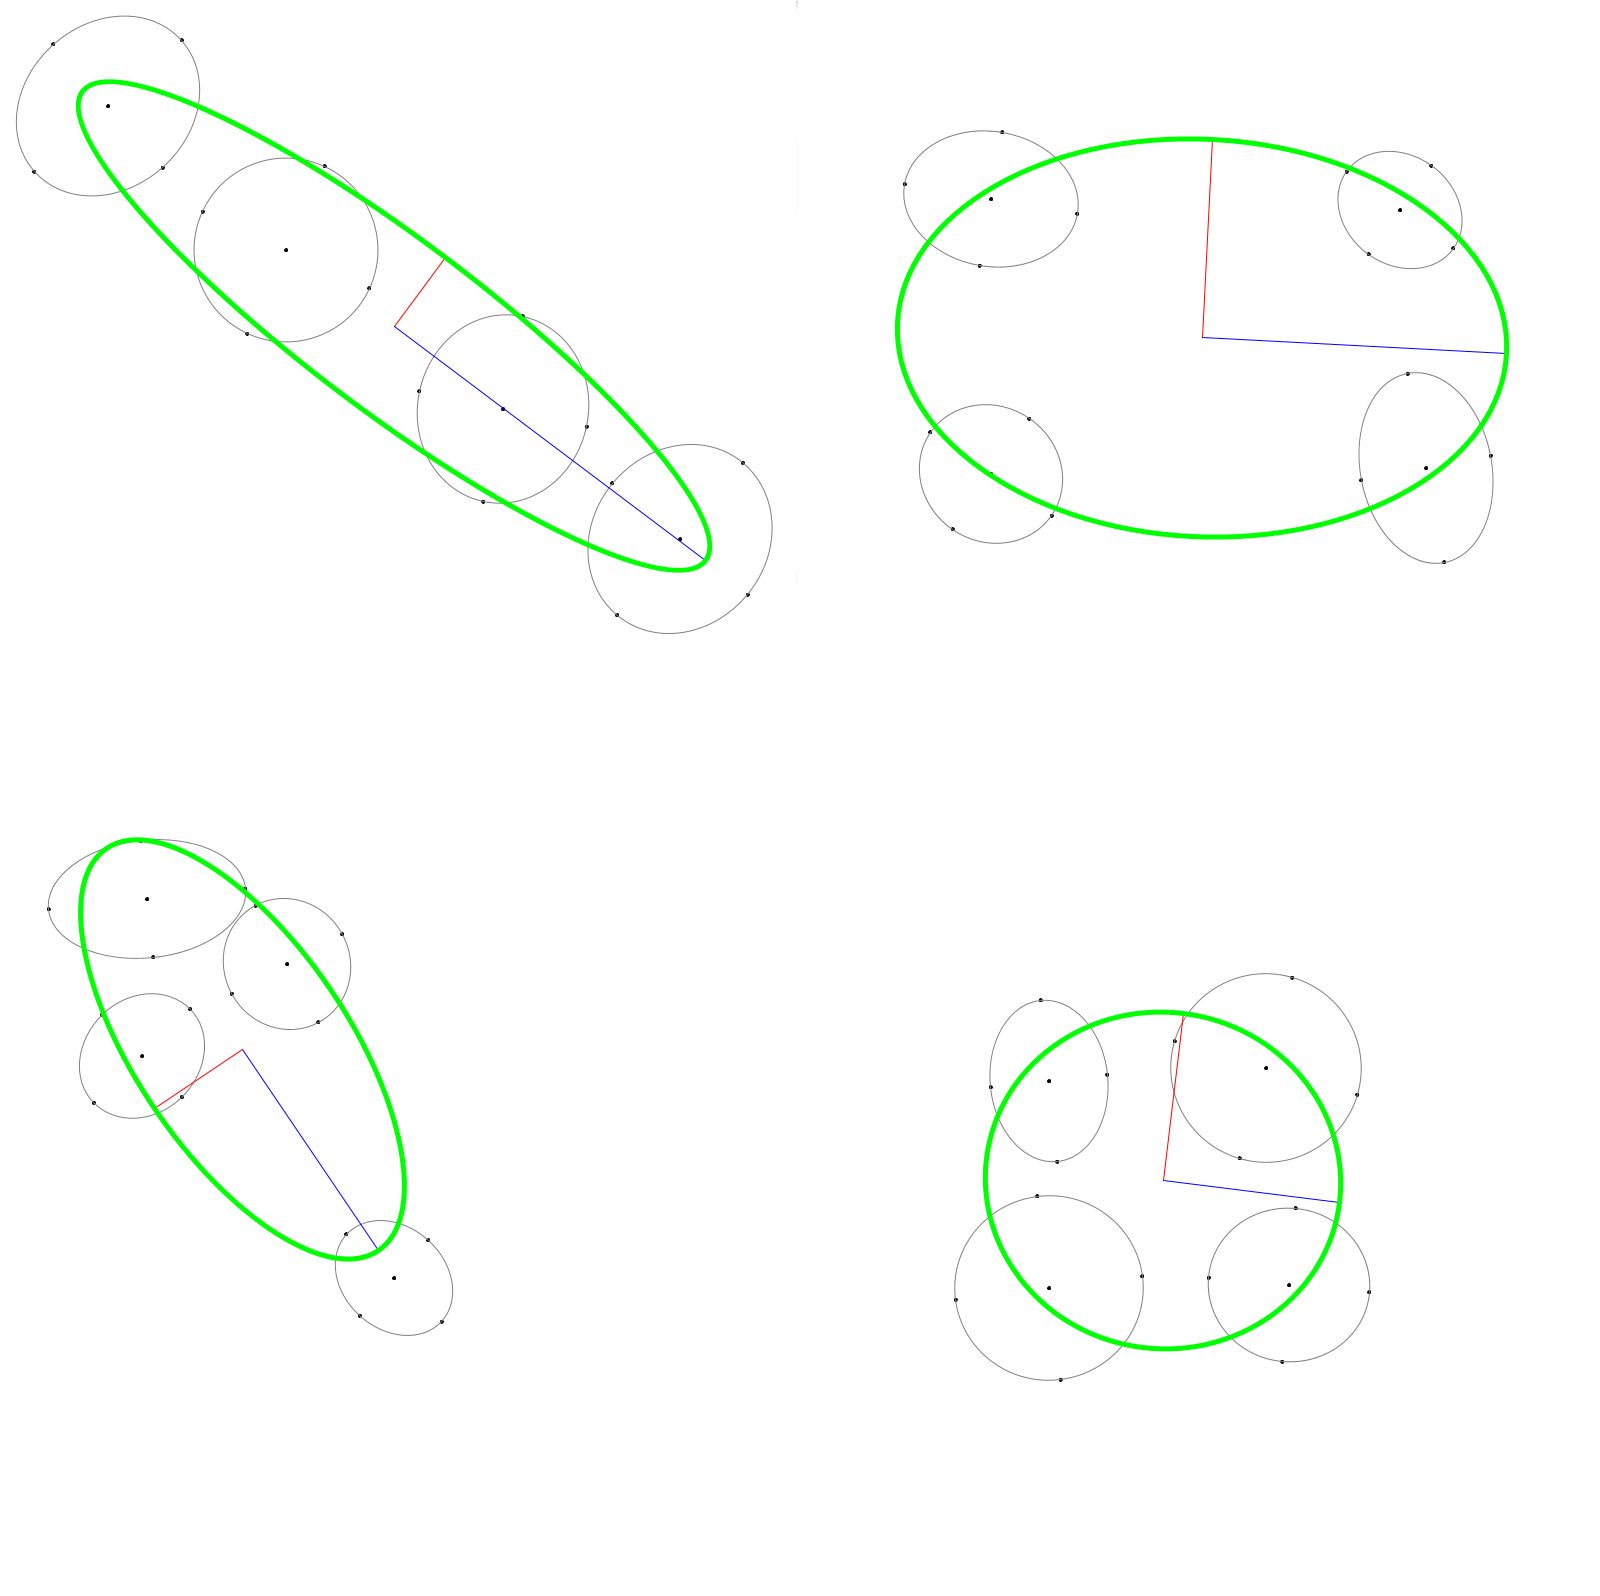
\includegraphics[width=0.7\linewidth]{figures/pca2d.png}
    \caption{Examples of computed point spread.}
    \label{fig:pca2d}
\end{figure}

The gray lines show the confidence ellipse of the initial Gaussians, and the dots show the distribution centers and ellipse vertices. The green line represents the confidence ellipse of the merged Gaussian, and the blue and red lines represent the covariance matrix eigenvalues. We can see that for Gaussians that are close together, the distribution spread follows the general shape. However, when the primitives are spread apart, the resulting merged Gaussian covers a significant amount of empty space. This highlights the necessity of a good selection mechanism for choosing the candidate Gaussians for merging. Ideally, we would like the primitive to be compact and without empty spaces between them.